\chapter{Virtualização}
\label{cap:virtualizacao}

O conceito virtualização surgiu na década de 60, onde muitas vezes havia a necessidade de um usuário utilizar um ambiente individual, 
com suas próprias aplicações e totalmente isolado dos outros usuários. Este foi um dos principais motivos para a criação de máquinas 
virtuais, mais conhecida como \ac{VM}, que teve forte expansão com um dos principais sistemas comerciais com suporte a virtualização, 
sistema operacional \textit{370} que foi desenvolvido pela \textit{IBM}. Este sistema operacional executava sobre \textit{mainframes}, 
que na época eram grandes servidores capazes de processar um grande volume de informações \cite{laureano2008}. 
%O conceito virtualização surgiu na década de 60, sendo que um dos principais motivos foi a necessidade de um grande servidor,
%conhecido como \textit{mainframe}, executar uma variedade de \textit{softwares}. Isso ocorreu pois cada \textit{mainframe} necessitava
%do próprio sistema operacional, pois cada \textit{software} possuia além da aplicação todo o ambiente operacional no qual executava. Assim
%sendo necessário a criação de máquinas virtuais, mais conhecida como \ac{VM} \cite{carissimi2008}.

Na década de 80, houve uma redução da utilização da virtualização devido a popularização do \ac{PC}. Na época era mais vantajoso disponibilizar 
um \ac{PC} para cada usuário, do que investir em \textit{mainframes}. Devido ao crescente avanço e melhor desempenho do \ac{PC} e
ao surgimento da linguagem \textit{Java}, no início da década de 90, a tecnologia de virtualização retornou com o conceito de virtualização
de aplicação.

A virtualização foi definida nos anos 60 e 70 como uma camada entre o \textit{hardware} e o sistema operacional que possibilitava a 
divisão e proteção dos recursos físicos. Porém, atualmente ela engloba outros conceitos, como por exemplo a \ac{JVM}, que não virtualiza
um \textit{hardware}. 

Atualmente define-se virtualização como uma camada de \textit{software} que utiliza os serviços fornecidos de uma determinada interface de 
sistema para criar outra interface de mesmo nível. Essa camada irá permitir a comunicação entre interfaces distintas, para suprir as 
necessidades dos componentes do sistema, de forma que uma aplicação desenvolvida para uma plataforma \textit{X} possa também executar 
em uma plataforma \textit{Y} \cite{laureano2008}. COLOCAR CONCEITO ISA

Máquinas virtuais podem ser divididas em dois grupos: máquinas virtuais de aplicação, detalhado na seção \ref{section:virtaplicacao}, e 
máquinas virtuais de sistema, detalhado na seção \ref{section:virtsistema}. A primeira faz a
virtualização de uma aplicação, suporta apenas um processo ou aplicação. 
A máquina virtual de sistema suporta sistemas operacionais convidados, com suas aplicações executando sobre ele \cite{laureano2008}.
//adicionar figura vm de processo e de sistema

\section{Máquinas virtuais de aplicação}
\label{section:virtaplicacao}
As máquinas virtuais de aplicação, também chamada de máquinas virtuais de processo, é geralmente conhecida por prover um ambiente
onde um sistema operacional suporte uma aplicação convidada, sendo que esta aplicação possui um conjunto de instruções diferentes
do sistema hospedeiro. Um exemplo disto é a \ac{JVM}, que permite a execução de aplicações \textit{Java} em diversos sistemas 
operacionais.

Na virtualização de aplicação também pode existir máquinas virtuais que utilizam as mesmas interfaces \ac{ISA} da máquina real,
com isso uma grande parte das instruções podem ser executadas diretamente, com exceção de instruções sensíveis, que serão devidamente
tratadas. Alguns tipos de máquinas virtuais de aplicação que utilizam as interfaces da máquina real são detalhadas abaixo:

\begin{itemize}
 \item Sistemas operacionais multi-tarefas
 
 \item Tradutores dinâmicos
 
As máquinas virtuais de aplicação mais populares hoje são aquelas em que a in-
terface binária de aplicação (ABI) requerida pela aplicação é diferente da oferecida pela
máquina real. Como a ABI é composta pelas chamadas do sistema operacional e as ins-
truções de máquina disponíveis à aplicação (user ISA), as diferenças podem ocorrer em
ambos. Nos dois casos, o hipervisor terá de realizar traduções dinâmicas (durante a exe-
cução) das ações requeridas pela aplicação em suas equivalentes na máquina real (como
visto, um hipervisor com essa função é denominado tradutor dinâmico).

 \item Depuradores de memória
 
\end{itemize}

Pode-se criar 

\begin{itemize}
 \item Máquinas virtuais de linguagem de alto nível
JVM Carrisimi
 \item Emulação no sistema operacional
Ex:
As máquinas virtuais de aplicação mais populares hoje são aquelas em que a in-
terface binária de aplicação (ABI) requerida pela aplicação é diferente da oferecida pela
máquina real. Como a ABI é composta pelas chamadas do sistema operacional e as ins-
truções de máquina disponíveis à aplicação (user ISA), as diferenças podem ocorrer em
ambos. Nos dois casos, o hipervisor terá de realizar traduções dinâmicas (durante a exe-
cução) das ações requeridas pela aplicação em suas equivalentes na máquina real (como
visto, um hipervisor com essa função é denominado tradutor dinâmico).
Caso as diferenças de interface entre aplicação e máquina real se restrinjam às
chamadas do sistema operacional, o hipervisor precisa apenas mapear as chamadas de
sistema usadas pela aplicação sobre as chamadas oferecidas pelo sistema operacional da
máquina real. Essa é a abordagem usada, por exemplo, pelo ambiente Wine, que permite
executar aplicações Windows em plataformas Unix. As chamadas de sistema Windows
emitidas pela aplicação em execução são interceptadas e transformadas em chamadas
Unix, de forma dinâmica e transparente (figura 4.12).
\end{itemize}


\section{Máquinas virtuais de sistema}
\label{section:virtsistema}



Virtualização de sistema utiliza abstração em sua arquitetura, por exemplo, ela transforma um disco físico em dois discos 
virtuais menores, sendo que esses discos virtuais são arquivos armazenados no disco físico. Sabendo que arquivos são uma abstração
em um disco físico, pode-se dizer que virtualização não é apenas uma camada de abstração do \textit{hardware}, ela faz a reprodução 
do \textit{hardware} \cite{smithenair2005}.

Um ambiente de virtualização de sistema é composto basicamente por três componentes:
\begin{itemize}
 \item Sistema real: também pode ser chamado de hospedeiro, que é o \textit{hardware} onde o sistema de virtualização irá executar;
 \item Camada de virtualização: é conhecida como hipervisor ou também chamado de \ac{VMM}, tem como função criar interfaces virtuais a
 partir de interfaces físicas para a comunicação do sistema real com o sistema virtual;
 \item Sistema virtual: também conhecido como \textit{guest}, ou sistema convidado, que executa sobre o sistema real. Geralmente
 existem vários sistemas virtuais executando simultaneamente sobre o sistema real.
\end{itemize}


\subsection{Hipervisores nativos}
\subsection{Hipervisores convidados}

\subsection{Virtualização de recursos}
\subsection{Virtualização completa}



\begin{figure}[acoplamento_interfaces]
 \centering
 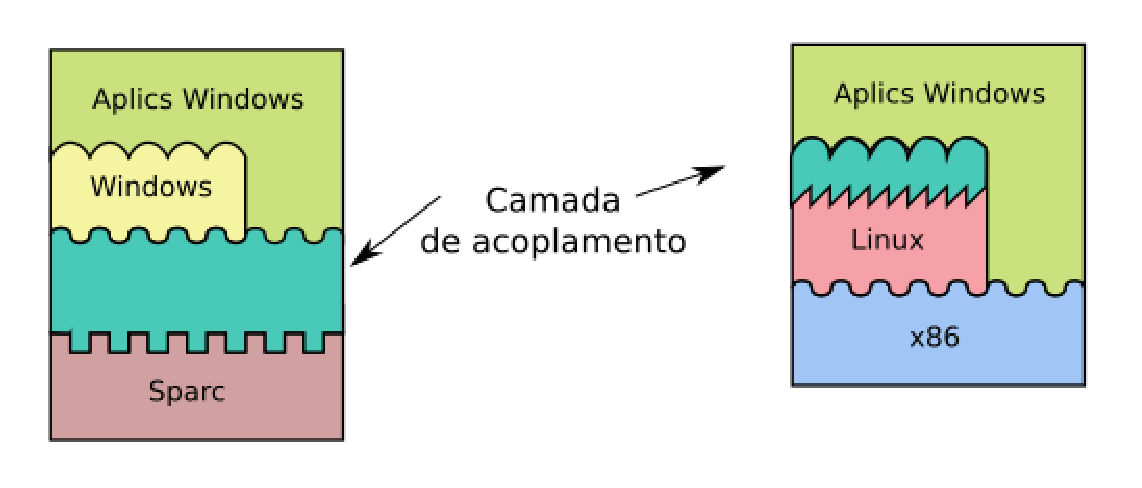
\includegraphics[height=140px]{img/acoplamento_interfaces.eps}
 \caption{Acoplamento entre interfaces distintas}
 \label{fig:acoplamento_interfaces}
 Fonte: \citet{laureano2008}
\end{figure}
Exemplo de camada de virtualização \ref{fig:acoplamento_interfaces} ....


Emulação????


\section{Vantagens}
\label{section:vantagensvirt}

Em muitos casos empresas utilizam serviços distribuídos entre servidores físicos, como, por exemplo, servidores de e-mail, hospedagens e 
banco de dados, com isso existe uma ociosidade grande de recursos. Portanto uma das grandes vantagens da virtualização é um melhor 
aproveitamento destes recursos, alocando vários serviços em um único servidor gerando um melhor aproveitamento do \textit{hardware} 
\cite{moreira2006}. Além disso, pode-se ter uma redução de custos com a administração e a manutenção dos servidores. Em um ambiente 
heterogênio pode-se também utilizar virtualização, pois ela permite a instalação de diversos sistemas operacionais em um único servidor.

Uma outra motivação para a utilização de virtualização consiste no custo da energia elétrica. A economia de energia pode ser obtida através 
da implantação de servidores mais robustos para substituir dezenas de servidores comuns. Outros fatores como refrigeração do ambiente e 
espaço físico utilizado também podem ser reduzidos com a implantação de virtualização de servidores, e consequentemente, reduzem os 
custos de energia também.

A virtualização favorece a implementação do conceito um servidor por serviço, que consiste em ter um servidor para cada serviço.
Mas porque não colocar todos serviços em um único servidor? Muitas vezes com uma variedade de serviços é necessário diferentes 
sistemas operacionais, ou os serviços necessitam rodar nas mesmas portas, portanto isto se torna inviável. Outro fator relevante que 
também favorece a implementação de um servidor por serviço é, caso exista uma falha de segurança em apenas um serviço, essa 
vulnerabilidade poderá comprometer todos os outros serviços 
\cite{carissimi2008}.


** Anéis de privilégios, compatibilidade, e hypervisor \cite{goncalves2009}.


%Virtualização_ da teoria a soluções.pdf
%virtualizacao mainframes: pag 1 - Alta Disponibilidade em Servidores Virtualizados.pdf
%pag 32 - Rejuvenescimento e migracao de vms - Matheus D'Eça de Melo.pdf
%pag 20 - Implementação de Alta disponibilidade em Máquinas Virtuais utilizando Software Livre.pdf
%ferramentas pag 4 - Main - Virtualização de serviços baseado em contêineres -WandersonReis.pdf

%Virtualizacao da teoria a solucoes:
%No entanto, essa abordagem trouxe como contra-partida a filosofia “um servidor
%por serviço”. Rapidamente, os responsáveis pelas áreas de TI se deram conta do
%problema (e custo) em gerenciar diferentes máquinas físicas, mesmo que tivessem o
%mesmo sistema operacional. Além disso, há problemas relacionados com consumo de
%energia elétrica, refrigeração, espaço físico, segurança física, etc. Nesse contexto, a
%virtualização surge como uma possibilidade de agregar os benefícios da componetização
%de sofware com a redução dos custos de manutenção de hardware e software. Assim, é
%possível manter a idéia de um “um servidor por serviço” sem ter um hardware
%específico.
%Essa abordagem é reforçada pela lei de Zipf [Adamic, 2008] que pode ser
%sintetizada da seguinte forma: a freqüência de um evento é proporcional a x −α , onde x é
%um ranking de comparação de um evento a outro. Alguns estudos [Breslau, Cao, Fan,
%Philips e Shenker, 2008] mostraram que a freqüência de acesso a servidores web e
%outros serviços Internet seguem uma distribuição Zipfian, o que, na prática, se traduz
%pelo fato de que a maioria dos acessos a serviços Internet é para uma minoria deles.
%Portanto, conclui-se que uma minoria de serviços está ativa enquanto a maioria está
%bloqueada a espera de requisições, o que, claramente, representa um desperdício de
%recursos. Para exemplificar, imagine, entre outros, o uso dos servidores de autenticação,
%DHCP, impressão, arquivos, e-mail, web e DNS em sua rede corporativa.

%Rejuvenescimento e migracao de vms:
%Com a arquitetura baseada em serviços, clientes podem utilizar serviços alocados em
%nuvem através dos web browsers. Unindo a computação em nuvem e a arquitetura baseada
%em serviços, aplicativos e demais recursos de TI podem ser oferecidos remotamente, como se
%estivessem localizados localmente. Vale a pena salientar que a arquitetura baseada em serviços
%permite monitorar em tempo real o uso dos recursos disponibilizados, colaborando assim para
%uma gerência mais eficiente a todo o sistema (LINTHICUM, 2009). Além disso, dependendo
%das interfaces definidas, pode-se ampliar consideravelmente o número de potenciais clientes.
%Recursos disponibilizados via navegador web, por exemplo, podem ser acessados tanto por
%computadores de mesa quanto por smartphones ou tablets.
%

%ver failover e failback em cluster?
